\chapter{In-depth Contrastive Error Analysis}
\label{chap:analysis}

% Length
% Graph factors
% Linguistic factors

% Peking: Ensemble method, combination of transition-based and graph-based
% Turku: Support Vector Machines
% Lisbon: A graph algorithm


In this chapter we will examine the results of SemEval-2015 for the Peking, Turku and Lisbon systems described in the previous chapter. The aim of this comparative analysis is twofold:

\begin{enumerate}
    \item To find differences in the results among a chosen set of parsing systems in order to compare and contrast their strengths and weaknesses.
    \item Empirically identify and verify which types of errors that can be the focus of future research on semantic dependency parsing.
\end{enumerate}

From such an analysis we want to examine if there is grounds to extrapolate from more fine grained observations to general ones, i.e. to make general assumptions based on the empirical observations. The three systems that we will examine: Peking, Turku, and Lisbon, have been chosen based on two factors:

\begin{enumerate}
    \item They are among the parsing systems with the highest overall scores in SemEval-2015. 
    \item The chosen parsing systems should are based on different algorithms, and include both the local transition-based and global graph-based models that we examined in Chapter \ref{chap:background}.
\end{enumerate}

We will argue that the analysis presented in this chapter can highlight the correlation between the specific types of errors that these parsers make and their theoretical foundation. The analysis presented is thus based on the general knowledge of the parsing systems, as described in Chapter \ref{chap:semantic}, and the specific observations made in our analysis of their results from SemEval-2015.

In our analysis we take inspiration from a similar study performed by \citeA{McD:Niv:07}, where a comparative analysis of a set of syntactic parsers has been performed. This study focuses on three types of errors: (1) length factors, (2) graph factors, and (3) linguistic factors. We will structure our analysis accordingly, and include a fourth type of errors that examine the multi-classification task of frame predication.

\section{Length factors}

As \citeA{McD:Niv:07} point out, it is well known that syntactic parsing systems produce results with lower accuracy for longer sentences. We observe the same phenomena in the results from our chosen set of parsers from SemEval-2015. Parsing accuracy is highly correlated with sentence length.

Another type of length factor is the length of dependencies, which also has an impact on the accuracy of predictions. We define the length of a dependency from word $w_i$ to $w_j$ as $j - i$. For the English language, and from examining the data sets used in SemEval-2015, we can generally state that short dependencies are modifiers of nouns, such as determiners, adjectives or pronouns. Longer dependencies are in most cases words that modify the main verb or root of the sentence. 

Both sentence and dependency length have a distribution in the data sets where the frequency of a length factor is correlated with the accuracy for parsing that specific length. The higher the frequency of a given length factor, the more likely that the parsing system has a higher accuracy when parsing a sentence or dependency with a given length. It is therefore important not to exaggerate the importance of the length factor itself, but rather the distribution with which it occurs in the data used for training. So a different data set and distribution would result in, if our assumptions are correct, parsing systems with a different correlation between length and accuracy. However, since we are dealing with natural language, we can also assume that a relatively similar distribution of sentence and dependency length that we observe in the SemEval-2015 data sets will occur in other corpora.

\section{Graph factors}

\section{Linguistic factors}

\section{Frames}

\subsection{Predicting frames}

\section{Conclusions}



% Input for graph images
% \begin{figure}[h]
% \caption{Caption}
% \centering
% 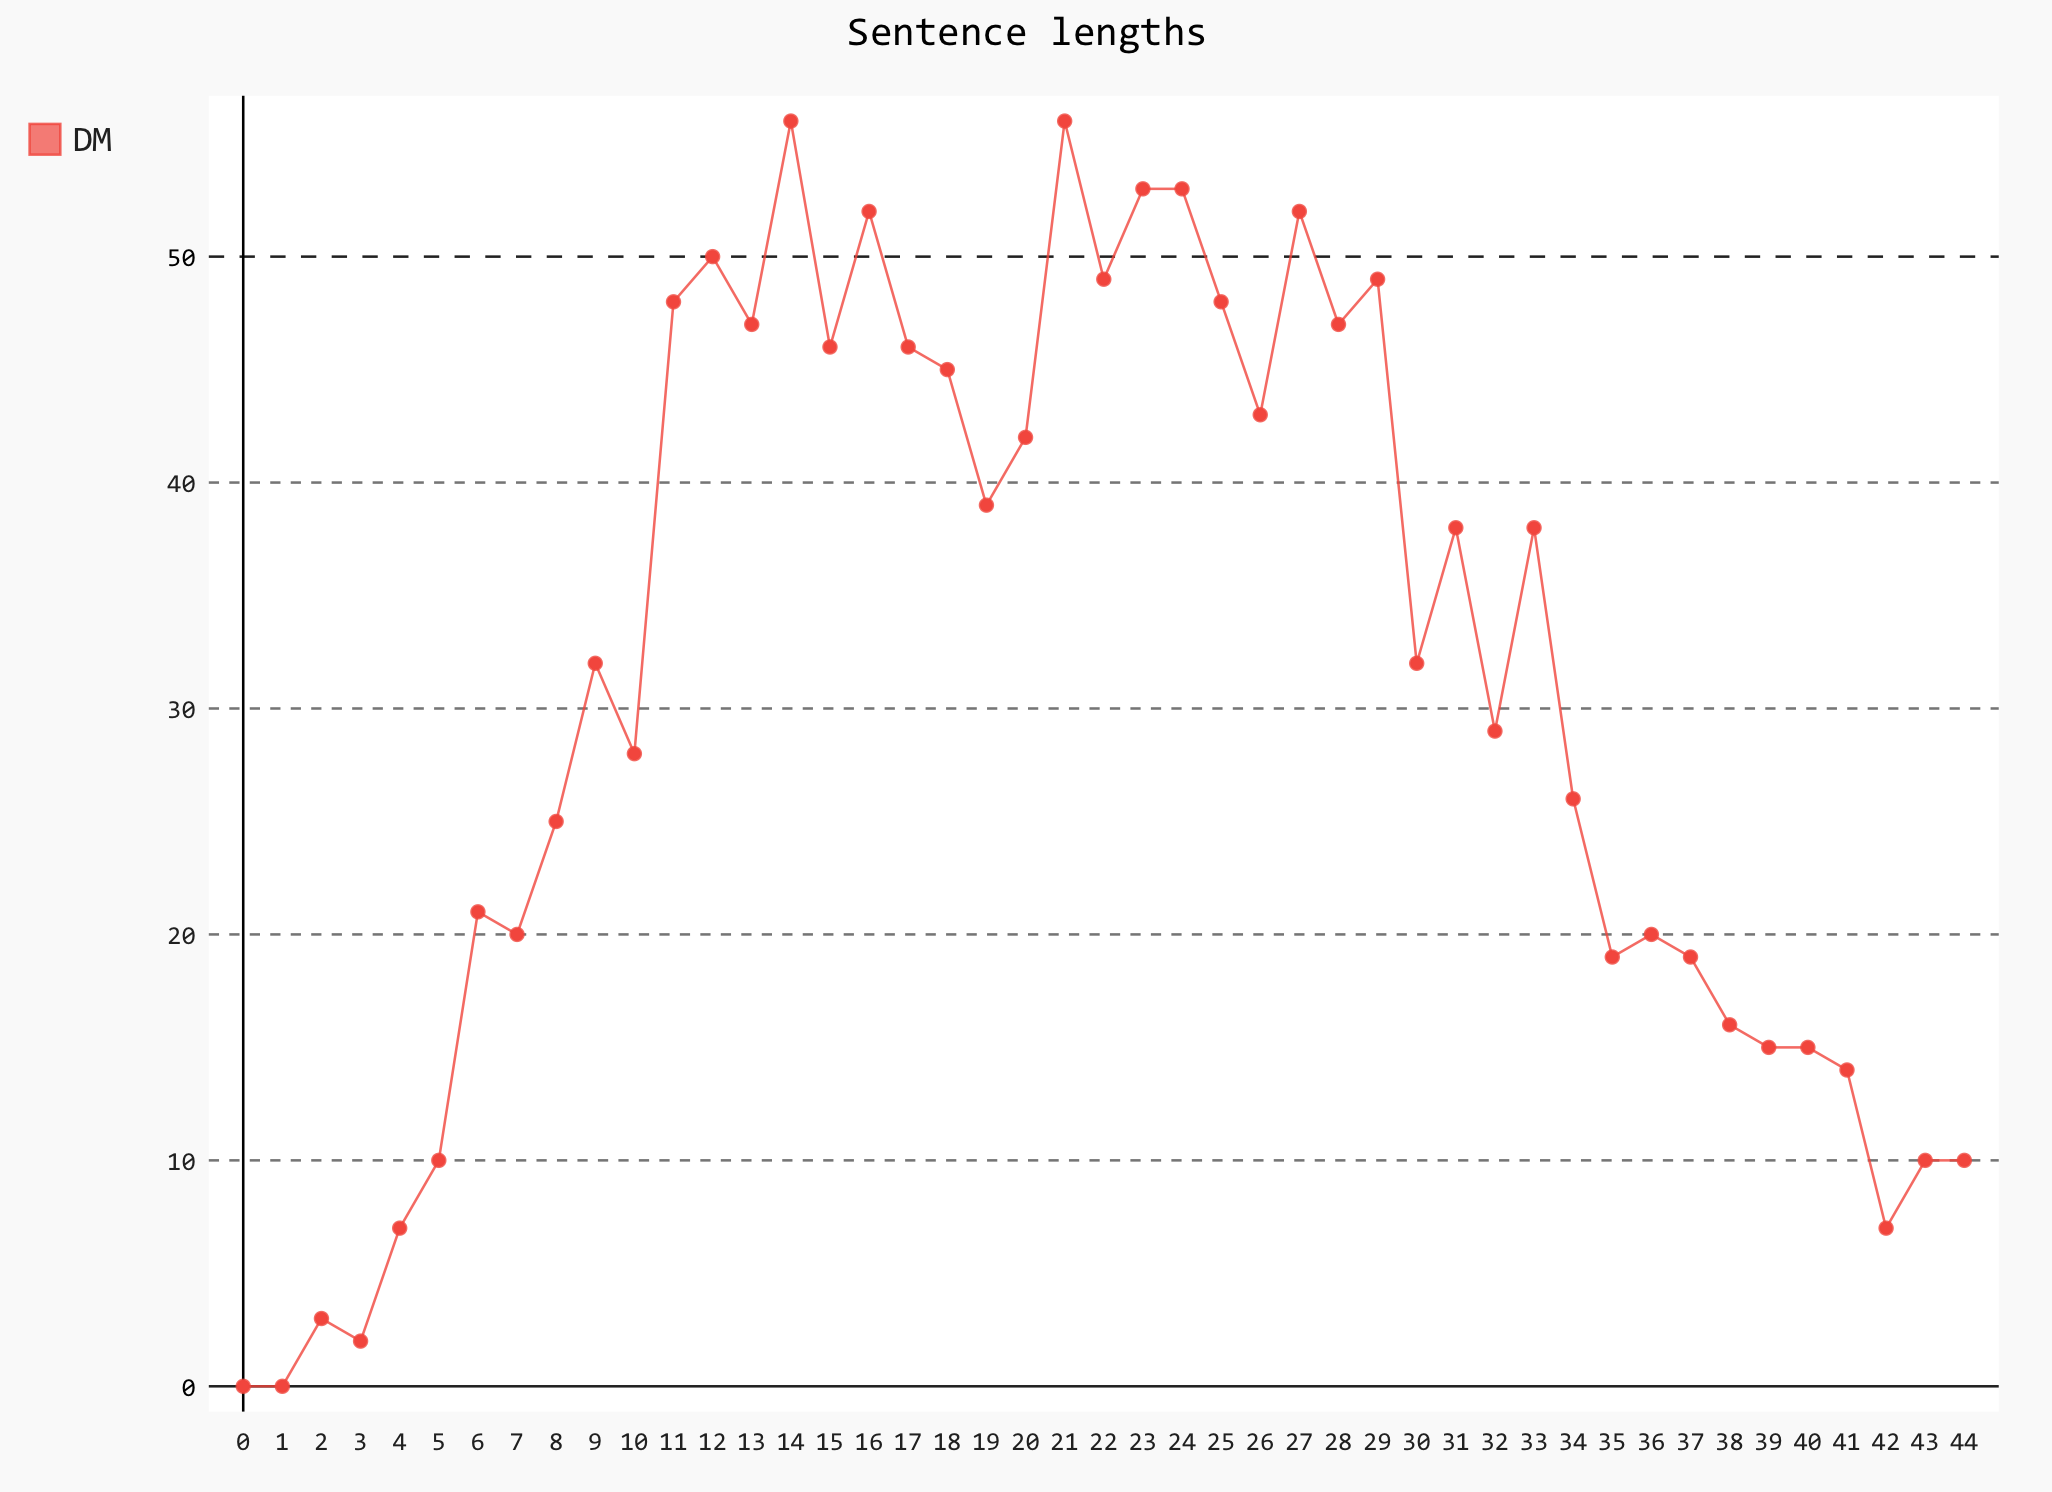
\includegraphics[width=\textwidth]{sentence_length}
% \label{fig:sentence_length}
% \end{figure}

